%	PACKAGES AND OTHER DOCUMENT CONFIGURATIONS

\documentclass[11pt, a4paper,twocolumn]{article} % 10pt font size (11 and 12 also possible), A4 paper (letterpaper for US letter) and two column layout (remove for one column) Use additional titlepage argument to generate this
%\documentclass[12pt, a4paper,twocolumn,titlepage]{article}

\input{structure.tex} % Specifies the document structure and loads requires packages
\graphicspath{{"/Users/Kit/OneDrive/Documents/Computing/Trojan Asteroids/Report/Figures"}}


%	ARTICLE INFORMATION

\title{Modelling the Trojan Asteroids}
%\subtitle{Blue Organic Light Emitting Diodes using Thermally Activated Delayed Fluorescence}

%\author{
	%\authorstyle{Christopher Gallagher}}
\author{\authorstyle{Christopher Gallagher} %Candidate 6952R}
	\institution{University of Cambridge}}
% Example of a one line author/institution relationship
%\author{\newauthor{John Marston} \newinstitution{Universidad Nacional Autónoma de México, Mexico City, Mexico}}

\date{\today} % Add a date here if you would like one to appear underneath the title block, use \today for the current date, leave empty for no date
\usepackage[english]{babel}
\usepackage{tabularx}
%\usepackage[backend=biber,doi=false]{biblatex}
\addbibresource{references.bib}
%\AtBeginBibliography{\small}

\usepackage{amsmath}
\usepackage{bm}
\usepackage{fixltx2e}% for \textsubscript


%----------------------------------------------------------------------------------------
\begin{document}

\maketitle % Print the title

\thispagestyle{firstpage} % Apply the page style for the first page (no headers and footers)

%	ABSTRACT

\lettrineabstract{Trojan asteroids orbit the Sun in resonance with Jupiter at Lagrange points,
	and have their own stable orbits about these points. This can be treated as a restricted three-body problem, which is numerically evaluated in this report using a stiff Radau method to solve the system of coupled differential equations. Without perturbations, a maximal deviation of 4.68\pmb{$\times$}10\pmb{$^{-13}$} AU  from the Lagrange points was observed over 1000 orbits (11,852 years). The application of perturbations to these asteroids demonstrated the predicted existence of stable tadpole and horseshoe orbits, and suggested that wander from the Lagrange point depends quadratically on perturbation size. Such orbits were observed to be stable up to a planetary mass of 0.04 \pmb{$M_{\odot}$}, also in agreement with theoretical predictions. Word Count: XXXX}


%	ARTICLE CONTENTS

%Use https://leancrew.com/all-this/2016/08/lagrange-points-redux/ to create your own contour plot?
\section{Introduction}
The Jupiter Trojans, commonly known as the Trojan asteroids, are two large groups of asteroids that share the planet Jupiter's orbit around the Sun in a 1:1 orbit resonance. These two groups are called the Greeks and the Trojans, named after opposing sides in the mythological Trojan war, and lead/trail Jupiter respectively in its orbit. They correspond to Jupiter's two stable Lagrange points: L\subscript{4}, lying 60° ahead of the planet in its orbit, and L\subscript{5}, 60° behind, with asteroids distributed in two elongated, curved regions around these Lagrange points. 

The first Jupiter Trojan, 588 Achilles, was discovered in 1906 by the German astronomer Max Wolf \cite{Nicholson1961}, and a total of 7642 Jupiter Trojans have been found as of February 2020 \cite{IAU2020}.

Research into Jupiter's Trojan asteroids continues, with the particular focus on their origins reliant on an understanding of their orbit stability \cite{DiSisto2019} \cite{Nesvorn2018}. This informs studies into their composition \cite{Brown2016}, as travel to these asteroids is considered for their potential in mineral mining \cite{Okada2017} \cite{Levison2016}. 

The purpose of this report is to use numerical simulation techniques to investigate the stability of orbits about the Lagrange points, demonstrating that asteroids oscillate about these points with small perturbations and quantifying the absolute distance of the asteroids from the Lagrange point (the wander) during their orbits. The impact of variation in planetary/solar mass on asteroid orbit stability will also be considered. 

% \cite{Nakamura2008} gives spatial distribution

\section{Theoretical Background}

\subsection{Lagrange Points} \label{lagrange}
The asteroids exist at or near Lagrange points, defined in Lagrange's initial analysis of the three-body problem in 1772 \cite{Lagrange1772}, in which he demonstrated the existence of five equilibrium points for an object of negligible mass orbiting under the gravitational effect of two larger masses. Three of these equilibrium points, L\subscript{1}\textendash L\subscript{3} lie on the line joining the two masses, while each of the remaining two points, L\subscript{4} and L\subscript{5}, lie at the apex of an equilateral triangle with base equal to the separation of the two masses (see Figure \ref{fig:lagrangepoints}). Although these points are all potential maxima, stable motion is possible around L\subscript{4} and L\subscript{5} due to the Coriolis force \cite{Lissauer2014}.
%lissauer also says stability is provided that the most massive body has at least 25 times the mass of the secondary

\begin{figure}[h]
	\centering
	\includegraphics[width=\linewidth]{Figures/lagrange_points}
	\caption{The location of the five Lagrange equilibrium points in the circular-restricted three-body problem. The solar and planetary masses are denoted by the large and small filled circles, and the letters P, H, and T denote passing, horseshoe, and tadpole orbits respectively. Note that the two massive bodies form an equilateral triangle with each of the L\subscript{4} and L\subscript{5} points. Reproduced from Marzari et al. \cite{Marzari2002}}
	\label{fig:lagrangepoints}
\end{figure}

Figure \ref{fig:lagrangepoints} depicts orbits about L\subscript{4} and L\subscript{5} (known as tadpole orbits), as well as horseshoe orbits between Lagrange points, described by Murray et al. \cite{Murray1999}.

This report will focus on tadpole orbits, a well-documented feature of Trojan orbits \cite{Garfinkel1983} \cite{Dermott1981} and of the restricted three-body problem in general. Their distinctive shape results from a long-period motion about the equilibrium point combined with a short-period oscillation due to the Keplerian motion of the asteroid. 

Szebehely et al. \cite{Szebehely1969} predict that this short period tends to the planetary period in the small planetary mass limit, while the long period is given by

\begin{equation}
T_{long} = T_{P} \sqrt{\frac{4}{27 \mu_{2}}}  
\end{equation}

where $\mu_{2} = m_{2} / (m_{1} + m_{2})$ and $ T_{P} $ is the period of planetary orbit.

\subsection{Theoretical Model} \label{theory}
The three-body problem, where the dynamics of three interacting bodies are determined from their initial positions and velocities, has no analytical (closed-form) solution in the general case \cite{Barrow2008}.

In this report, I will consider the circular, restricted, three-body problem, where two of the bodies move in circular, coplanar orbits about their common centre of mass (CoM), unaffected by the negligible mass of the third body. I will also assume that all interactions are via Newtonian gravity.

The system of differential equations determines the position and velocity of the asteroids, with two equations per spatial coordinate.
\begin{equation}
\frac{dr_{i}}{dt} = v_{i}, \frac{dv_{i}}{dt} = g_{i}, \quad i = x,y 
\end{equation}

In this, $g_{i}$ is given by:
\begin{equation}
\textbf{g}= - \frac{G M_{s}}{\lvert \textbf{r} - \textbf{r}_{s} \rvert ^{3}} (\textbf{r} - \textbf{r}_{s})
		 - \frac{G M_{p}}{\lvert \textbf{r} - \textbf{r}_{p} \rvert ^{3}} (\textbf{r} - \textbf{r}_{p})
\end{equation}
where the subscripts \textit{s} and \textit{p} refer to solar and planetary properties respectively.

We may also consider a frame rotating at the same velocity as the massive bodies. As there is 1:1 orbital resonance between Jupiter and the asteroids, all three bodies are stationary in this frame. This significantly increases the accuracy of numerical simulations, as the exact solution is stationary with no explicit time dependence, rather than requiring an infinite power series \cite{Guglielmi2001}, \cite{LeVeque2007}.

When transforming into this rotating non-inertial frame, $g_{i}$ gains an additional virtual force term with coupling between the spatial coordinates. This is given below as the sum of the centripetal and Coriolis forces:

\begin{equation}
\Delta g_{i} = \Omega^{2} r_{i} - 2[\bm{\Omega} \times \textbf{v}]_{i}
\end{equation}
where $\Omega$ is the angular speed of the rotating frame, and $\textbf{v}$ is the velocity of the asteroid within this frame. 


\subsection{Symmetry} \label{symmetry}
This problem contains a number of symmetries, which were employed to simplify the problem and reduce the computational load. The Trojan and Greek asteroids are in equivalent positions, so experience the same forces, and the system has rotational and inversion symmetry, so the choice of initial point and orbit direction is arbitrary. Therefore, only the Greeks, orbiting counter-clockwise with perturbations applied at t = 0, need be considered.

\subsection{Orbit Geometry}
As the three bodies considered here form an equilateral triangle in the initial equilibrium state, as depicted in Figure \ref{fig:geometry}, we can easily derive the polar coordinates of each body with respect to the centre of mass about which the bodies orbit.

\begin{figure} %place in text?
	\centering
	\resizebox{\columnwidth}{!}{%
		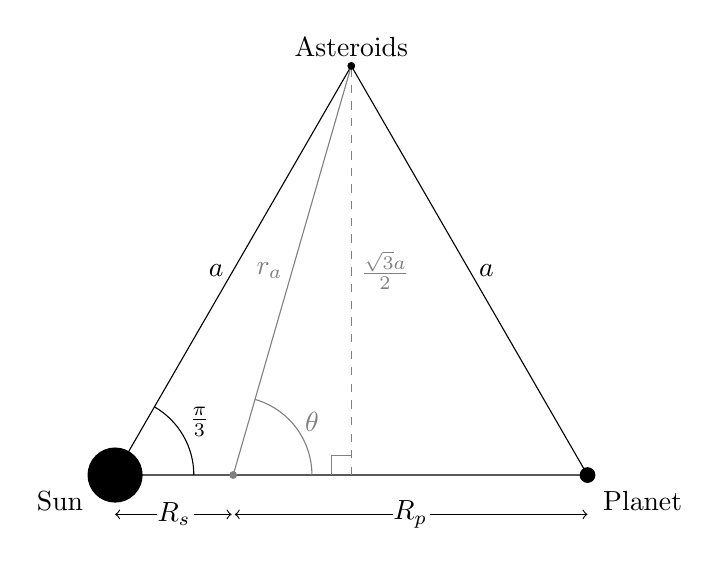
\begin{tikzpicture}
		\draw (0,0) -- (6,0) -- (3, {6*sin(60)} ) node[above]{Asteroids} node[midway,right]{$a$} -- cycle node[midway,left]{$a$};
		\draw  (1,0) arc (0:60:1cm)  ;
		%\node [label={[shift = {(10mm,5mm)}]{$\frac{\pi}{3}$}}] {};
		\node [label={[shift = {(13:11mm)}]{$\frac{\pi}{3}$}}] {};
		\node [label={[shift = {(-7mm,-7mm)}]{Sun}}] {};
		\node [label={[shift = {(67mm,-7mm)}]{Planet}}] {};
		
		\fill[gray] ({6*(1/4)}, 0) circle (0.5mm);
		\draw[gray] ({6*(1/4)}, 0) -- (3, {6*sin(60)} ) node[midway,left]{$r_{a}$};
		\draw[dashed, gray] (3, 0) -- (3, {6*sin(60)} )node[midway,right]{$\frac{\sqrt{3}a}{2}$};
		\draw[gray]  ({6*(1/4) + 1}, 0) arc (0:{atan(4*sin(60))}:1cm)  ;
		\node [label={[gray, shift = {(25mm,3mm)}]$\theta$}] {};
		\draw[gray] (2.75,0) -- (2.75, 0.25) -- (3, 0.25);
		
		\draw[arrows=<-](0,-0.5)--(0.53,-0.5);
		\node at (0.75, -0.5) {$R_s$};
		\draw[arrows=->](1.0,-0.5)--(1.48,-0.5);
		
		\draw[arrows=<-](1.52,-0.5)--(3.53,-0.5);
		\node at (3.75, -0.5) {$R_p$};
		\draw[arrows=->](4.00,-0.5)--(6,-0.5);
		
		%\draw[arrows=<-](0,-1)--(2.88,-1);
		%\node at (3, -1) {$a$};
		%\draw[arrows=->](3.1,-1)--(6, -1);
		
		\fill[black] (0,0) circle (3.5mm);% node[anchor=north west] {Sun};
		\fill[black] (6,0) circle (1mm);
		\fill[black] (3, {6*sin(60)} ) circle (0.5mm);
		
		\end{tikzpicture}
	}	
	\caption{A geometric depiction of the three-body system, in the case where the planet has a mass equal to one-third of the sun, and asteroids are considered at the L\subscript{4} point. $ R_{s} $ and $ R_{p}$ denote the (fixed) radii from the centre of mass (the grey point) to the Sun and the planet respectively, while $ r_{a} $ denotes the radius of the asteroids.}
	\label{fig:geometry}
\end{figure}

Using standard trigonometric relations, it is simple to show that the values $ r_{a} $ and $ \theta $ are given by:

\begin{equation}
r_{a} = \sqrt{a^{2} + R_{s} R_{p}} , \enspace \theta =  \tan^{-1} \left( \frac{a \sin(\frac{\pi}{3})}{R_{p} - \frac{a}{2}} \right)
\end{equation}

Furthermore, the Lagrange point in Cartesian coordinates based about the CoM is easily found to be:

\begin{equation}
(x,y) = \left( R_{p} - \frac{a}{2}, \frac{ \sqrt{3} a}{2} \right)
\end{equation}

Finally, equating the gravitational and centripetal forces on the planet allows the derivation of its (and all other bodies') orbital velocity:

\begin{equation} \label{frequency}
\Omega = \sqrt{\frac{G (M_{s} + M_{p})}{a^{3}}}
\end{equation}

\section{Methodology}
This system of coupled first-order ordinary differential equations (ODEs) was solved using the scipy \textit{solve\_ivp} function. The time span was taken as 100 orbits (with 100 points sampled per orbit) unless otherwise stated; this corresponds to 1185 Earth years. Rescaled solar system units are used for mathematical ease, so distances are measured in astronomical units (AU), time in Earth years and mass in multiples of the solar mass, to prevent floating point overflows due to the magnitude of the quantities considered in SI units.

The wander was defined as the maximum distance of the asteroid from the initial point during the orbit (for small perturbations this is also approximately the separation from the Lagrange point). Initial conditions are defined by the Lagrange point in each frame, with the initial velocity in the stationary frame defined by the period of Jupiter's orbit, and split into Cartesian components.

\subsection{Integration Method}
Within \textit{solve\_ivp}, the default solver is RK45 (an explicit Runge-Kutta method of order 5(4) \cite{Dormand1980}) which gives a deviation in asteroid position (from the Lagrange point) in the order of $ 10^{-4}$ AU in the rotating frame over 50 orbits. This is larger than expected, suggesting that the system of equations may require an unreasonably small step-size for numerical stability in this method, even in regions where the solution curve is smooth \cite{Lambert1991}. Such systems are known as stiff, and solvers designed for these systems typically do more work per step, allowing them to take much larger steps, and have improved numerical stability compared to non-stiff solvers, such as RK45 \cite{Byrne1987}. 

Therefore the stiff Radau solver (an implicit Runge-Kutta method from the Radau IIA family of order 5 \cite{Hairer2010}) is used for increased stability \cite{Frank1985}, and achieves a deviation in asteroid position in the order of $ 10^{-13}$ AU instead. This also ensures stability in the stationary frame, with deviations of 0.76\% in asteroid separation from Jupiter over $ 10^{3} $ years, compared to 53\% for the best non-stiff solvers.

%Can add more detail on A vs B stability (I believe B stability is relevant here but maybe check this)

\subsection{Programme Structure}
Global constants, such as solar mass, and sun\textendash planet separation, along with derived values from these, such as orbital period and solar radius from the CoM, are given in an importable python module, "\textit{constants}".

Functions to evaluate these coupled differential equation systems are defined in the module "\textit{orbits}", while additional functions to evaluate the wander during the orbit (under different sampling routines) are implemented in "\textit{wander}". Complete code listings for these files are given in Appendix \ref{Code}. Further files then import these modules and produce the plots given in this report, fully detailed in Appendix \ref{structure}.

When varying planetary mass, I considered it preferable to avoid reconstructing all functions to take planetary mass as an argument, as this requires re-evaluating all initial derived constants in the "\textit{orbits}" module. Therefore, I iterate over alternative planetary masses, re-defining constant values in each instance, and directly import the required functions to compute the orbit. 


\subsection{Performance} \label{Performance}
Sampling 100 points per orbit for 100 orbital periods takes a mean time of $16.97 \pm 34$ \si{\milli\second}, with sub-linear scaling for sampling rate and approximate linear scaling with orbit number up to the array memory limit, achieved through the optimised integration routines within \textit{solve\_ivp}. Computing the wander over position/velocity space with larger perturbations was, however, more time consuming, averaging $2.04 \pm 0.16$ \si{\second} per point with the same parameters. 

The main computational load was within the \textit{solve\_ivp} function, which is already optimised well beyond the capabilities of the author. However, assumptions made in Section \ref{symmetry}, such as considering only one group of asteroids, reduces this time somewhat, and vectorisation of other aspects of the \textit{orbit} functions reduced the running time of the whole module. These approaches were not taken universally however, due to the size of the arrays required, and the dominant effect of the ODE solver on the running time; instead, the orbit number was reduced when only a comparison of the maximum wander was required. 

\subsection{Fourier Analysis} \label{Fourier}
For periodic oscillations and orbits, the Fast Fourier Transform (FFT) implemented in \textit{scipy} is used to obtain the period, with \textit{find\_peaks} in \textit{scipy.signal} identifying the exact values. The errors were estimated using the associated peak widths of each frequency component.

\section{Results}
\subsection{Unperturbed Stability of Lagrange Points} \label{unperturbed}
Without perturbations applied, the Greeks' orbit has a maximum deviation from L\subscript{4} of $4.68 \times 10^{-13}$ AU over 100 orbits (1185 years). This value is unchanged if 1000 orbits are considered instead, confirming the stability of this Lagrange point.

In the stationary frame, this wander from the (now moving) Lagrange point is depicted in Figure \ref{fig:greeksdeviationstationaryframe}. The wander oscillates with a magnitude of $9.10 \times 10^{-2}$ AU, over a period of $148 \pm 4$ years. This is modulated with a faster oscillation component of $11.85 \pm 0.27$ years, equivalent to the orbital period of the asteroids.

\begin{figure}
	\centering
	\includegraphics[width=\linewidth]{Figures/greeks_deviation_stationary_frame}
	\caption{The wander of Greek asteroids from the Lagrange point in the stationary frame. Note the two oscillation components and constant maximum oscillation amplitude over time, demonstrating this point is indeed stable.}
	\label{fig:greeksdeviationstationaryframe}
\end{figure}

These much more significant deviations are due to time-dependence in the exact solution, as detailed in Section \ref{theory}. Energy can also be evaluated, and conserved, in this inertial frame; asteroid specific energy varies within only 0.113\% of the initial value, and with a similar periodicity to wander. Energy is also negative, confirming the asteroids are located within a bound orbit.

Animations produced to demonstrate the orbit in the stationary frame are included in Supplementary Material I-II. Animation I depicts the orbit as evaluated by the Radau solver, while II depicts it with LSODA, demonstrating the drift present over time with non-stiff solvers.

\subsection{Wander Analysis} \label{perturbed}
Wander from the initial point was calculated for random perturbations with a maximum magnitude of 1\% of the displacement from the origin. The perturbation components parallel and perpendicular to the position vector from the CoM (hereafter referred to as radial and tangential components respectively) were considered separately. By considering these perturbations across position space, it was clear that the wander is fully determined by the radial component, with no tangential dependence (as shown in Figure \ref{fig:wanderplots}).


\begin{figure}[ht]
	\centering
	\begin{subfigure}{.45\textwidth}
		\centering
		% include first image
		\includegraphics[width=\linewidth]{Figures/wanderagainstradialpertubation2}  
		\caption{Radial}
		\label{fig:wander_rad}
	\end{subfigure}
	\hfill %% useful if width of each figure is less the .5\textwidth
	\begin{subfigure}{.45\textwidth}
		\centering
		% include second image
		\includegraphics[width=\linewidth]{Figures/wanderagainsttangentialpertubation2}  
		\caption{Tangential}
		\label{fig:wander_tan}
	\end{subfigure}
	\caption{Wander from an initial perturbation with maximum relative magnitude of 0.1\% of the displacement from the origin, given in radial and tangential directions.}
	\label{fig:wanderplots}
\end{figure}

Figure \ref{fig:wander_rad} demonstrates a polynomial dependence on perturbation size in the radial direction, with a negligible constant term. While a quadratic has been fitted here, the possibility of higher order terms could not be eliminated, as increasing perturbation size beyond 0.06 AU can lead to unstable orbits.

We may consider the wander resulting from perturbations in position and velocity space. Figure \ref{fig:position_mesh} clearly shows dependence on radial position perturbations only, while Figure \ref{fig:velocity_mesh} shows a similar dependence on tangential velocity perturbations.

\begin{figure}[ht]
	\centering
	\begin{subfigure}{.45\textwidth}
		\centering
		% include first image
		\includegraphics[width=\linewidth]{Figures/testcolourmesh6}  
		\caption{Position}
		\label{fig:position_mesh}
	\end{subfigure}
	\hfill %% useful if width of each figure is less the .5\textwidth
	\begin{subfigure}{.45\textwidth}
		\centering
		% include second image
		\includegraphics[width=\linewidth]{Figures/testvelocitymesh2}  
		\caption{Velocity}
		\label{fig:velocity_mesh}
	\end{subfigure}
	\caption{Wander from an initial point in position and velocity space, only calculated over 50 orbits with 30 points per orbit to reduce computational load. Note the dependence on radial position and tangential velocity perturbation components. }
	\label{fig:mesh_plots}
\end{figure}

\subsection{Orbit Types} \label{orbits}
Figure \ref{fig:orbitplots} displays orbits resulting from small perturbations in the radial and tangential directions.

\begin{figure}[ht]
	\centering
	\begin{subfigure}{.23\textwidth}
		\centering
		% include first image
		\includegraphics[width=\linewidth]{Figures/radialp_orbits}  
		\caption{Radial}
		\label{fig:orbit_rad}
	\end{subfigure}
	\hfill %% useful if width of each figure is less the .5\textwidth
	\begin{subfigure}{.23\textwidth}
		\centering
		% include second image
		\includegraphics[width=\linewidth]{Figures/tangentialp_orbits}  
		\caption{Tangential}
		\label{fig:orbit_tan}
	\end{subfigure}
	\caption{Orbits from an initial perturbation of magnitude 0.01 AU from the origin, in radial and tangential directions, over 12 orbital periods. Note the tadpole features resulting from the radial perturbation, and the significantly larger wander than from the tangential perturbation.}
	\label{fig:orbitplots}
\end{figure}

The tadpole orbit in Figure \ref{fig:orbit_rad} consists of two oscillating components, as described in Section \ref{lagrange}. The short period, measured at $11.85 \pm 0.61$ years, is in excellent agreement with  planetary orbital period as expected; meanwhile the long period is measured to be $148 \pm 5$ years, consistent with the analytical value of $144$ years.

For a narrow range of larger perturbations, stable horseshoe orbits encompassing both Lagrange points may also be observed, as depicted in Figure \ref{fig:horseshoe}. This has a full period of $353$ years, in agreement with Taylor et al.'s numerical result of $358 \pm 7$ years \cite{Taylor1981}.

%smooth families of horseshoe-shaped longperiodic orbits for alpha2 > 1. Smooth, because they are restricted to shallow resonance, where the evolution of the epicyclic cusps and loops cannot be seen. - according to taylor, but havn't found smooth orbits here

\begin{figure}
	\centering
	\includegraphics[width=0.8\linewidth]{Figures/horseshoe}
	\caption{Horseshoe and tadpole orbits in the rotating frame, from radial perturbations of 0.07 and 0.01 AU respectively, over 30 orbital periods.}
	\label{fig:horseshoe}
\end{figure}

\subsection{Perturbations in Z direction} \label{3D}
Perturbations in the Z direction are aligned with the angular velocity vector for the rotating frame, so experience no virtual forces in this direction, and oscillate under the influence of gravity alone. Considering small perturbations in the Z direction (so that the distance from the CoM can be considered constant), the period of such oscillations tend to the orbital period of the rotating frame under Newtonian gravity, as detailed in Appendix \ref{zperiod}. These oscillations are observed to be approximately sinusoidal, with a measured period of $11.85 \pm 0.48$ years, in strong agreement with the theoretical predictions.

\begin{figure}
	\centering
	\includegraphics[width=0.8\linewidth]{Figures/z_perturbations5c}
	\caption{Variation of wander with increasing Z perturbations. A strong linear component is observed initially in the un-perturbed case, but then tends towards the perturbed quadratic case, while the linear offsets result from the initial perturbation in the XY plane.}
	\label{fig:zwander}
\end{figure}

The overall wander, however, is observed to follow Figure \ref{fig:zwander}.
It is suggested that, while the maximum deviation from the Lagrange point in the Z direction is simply twice the initial perturbation, wander in the XY plane increases quadratically. This can be initiated from a radial displacement due to the reduced gravitational force  under the Z perturbation, demonstrated in Figure \ref{fig:zorbit} or, more significantly, from an initial perturbation in the XY plane. However, the oscillation of gravitational forces due to perturbations in the Z direction make this problem significantly more complicated and are a possible cause of the observed deviations from the quadratic relations.

\begin{figure}
	\centering
	\includegraphics[width=0.8\linewidth]{Figures/z_perturb_orbit}
	\caption{Orbit of Greek asteroids following a 0.2 AU perturbation in the positive Z direction, over 12 orbital periods. Note the initial outwards radial displacement despite the lack of perturbation in the XY plane, and subsequent tadpole-like orbit.}
	\label{fig:zorbit}
\end{figure}

\subsection{Variation of Planetary Mass} \label{planet}
The variation of wander with planetary mass is given in Figure \ref{fig:planetmass}.

\begin{figure}
	\centering
	\includegraphics[width=0.8\linewidth]{Figures/wanderwithplanetmass_q7}
	\caption{Variation of maximum wander with planetary mass, under a 0.001 AU radial perturbation and 0.001 AU/year tangential boost. Note the tendency }
	\label{fig:planetmass}
\end{figure}

For small planetary masses (up to approximately $ M_{p} = 0.01 M_{s}$), the wander follows a $ M_{P}^{-\frac{1}{2}}$ dependence, tending towards the initial perturbation for larger masses. However, wander increases unbounded and orbits become unstable beyond $ M_{p} = 0.04 M_{s}$, as depicted in Figure \ref{fig:planetmass2}, in agreement with theoretical predictions by Darwin \cite{Darwin1897}.

\begin{figure}
	\centering
	\includegraphics[width=0.8\linewidth]{Figures/wanderwithplanetmass_p6}
	\caption{Variation of maximum wander with planetary mass, under a 0.01 AU radial perturbation and 0.01 AU/year tangential boost. Note the orbit stability up to $ M_{p} = 0.04 M_{s}$, and instability beyond this.}
	\label{fig:planetmass2}
\end{figure}

\section{Conclusion}
This report demonstrates the stability of Lagrange points L\subscript{4} and L\subscript{5}, with a maximum deviation from the Lagrange points of $4.68 \times 10^{-13}$ AU over 1000 orbits (11,852 years), in a frame rotating with the asteroids and without perturbations applied. Stability under perturbations in both the XY plane and in the Z direction is also demonstrated, with a finite wander from these points independent of orbit duration. It was possible to further quantify this wander, suggesting a strong quadratic dependence on radial perturbation magnitude and independence of tangential perturbations, which did not grow beyond the initial perturbation size.
It was also possible to replicate both tadpole and horseshoe orbits from radial perturbations, and frequency components were obtained for these orbits in agreement with previous literature. It was also found that orbits become unstable when the planetary\textendash solar mass ratio is greater than 0.04, in agreement with theoretical predictions, and inverse root mass dependence below this point.

Further work is required to evaluate coefficient values for polynomial relationships observed, and to demonstrate a theoretical basis for such dependencies.
Further research would also be beneficial on the categorisation of different orbit types, and examination of initial conditions corresponding to formation mechanisms of these orbits. 



\clearpage
\printbibliography

\onecolumn
\begin{appendices}
\section{Z Perturbation Period} \label{zperiod}
Figure \ref{fig:geometryz} depicts a Z perturbation out of the XY plane, from the L\subscript{4} point.
\begin{figure} [h]
	\centering
	\resizebox{0.5\columnwidth}{!}{%
		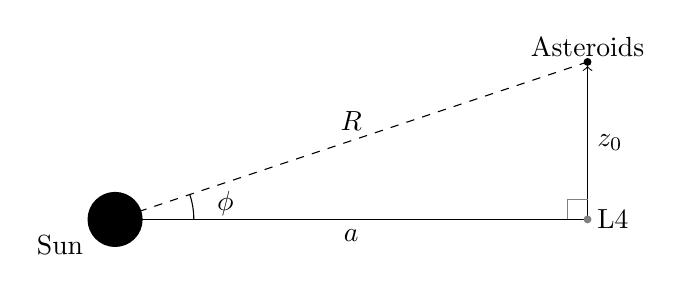
\begin{tikzpicture}
		\draw (0,0) -- (6,0)  node[midway, below]{$a$} node[right]{L\subscript{4}}; 
		\draw [arrows=->] (6,0) --  (6, 1.95 ) node[above]{Asteroids} node[midway,right]{$z_{0}$};
		\draw [dashed] (6,2) -- (0,0) node[midway, above]{$R$};
		\node [label={[shift = {(-7mm,-7mm)}]{Sun}}] {};
		\fill[black] (0,0) circle (3.5mm);% node[anchor=north west] {Sun};
		\fill[black] (6,2) circle (0.5mm);
		\fill[gray] (6,0) circle (0.5mm);
		
		
		\draw  (1,0) arc (0:{atan(1/3)}:1cm)  ;
		\node [label={[shift = {(14mm,-2mm)}]{$\phi$}}] {};
		\draw[gray] (5.75,0) -- (5.75, 0.25) -- (6, 0.25);
		\end{tikzpicture}
	}	
	\caption{A geometric description of asteroids at the L\subscript{4} point undergoing a perturbation of magnitude $z_{0}$ out of the XY plane. The fixed equilibrium distance between the asteroids and the Sun is denoted by $a$, while $R$ represents the separation between the asteroids and the Sun as a result of the perturbation} 
	\label{fig:geometryz}
\end{figure}

As the asteroid is equidistant from the Sun and the planet, the magnitudes of these forces depend on these bodies' mass only, and gravitational force components from both massive bodies are similarly orientated in the Z direction. The total gravitational force acting on the asteroid is therefore given by:

\begin{equation}
F = - \frac{G (M_{s} + M_{p}) M_{a}}{R^{2}}
\end{equation}
	
where $M_{s}$, $M_{p}$ and $M_{a}$ represent the solar, planetary and asteroid masses respectively. Resolving this force in Cartesian components, the Z component is given by:

\begin{equation}
F_{z} = F cos(\phi) = F \frac{z}{R} = - \frac{G (M_{s} + M_{p}) M_{a} z}{R^{3}}
\end{equation}

In conjunction with Newton's Second Law, we therefore obtain a second order differential equation for $z$:

\begin{equation}
\ddot{z} + \frac{G (M_{s} + M_{p})}{R^{3}} z = 0
\end{equation}
	 
which can be treated as simple harmonic motion in the small perturbation limit where $R \approx a$. This has a angular frequency equal to (\ref{frequency}):

\begin{equation}
\Omega = \sqrt{\frac{G (M_{s} + M_{p})}{a^{3}}}
\end{equation}

\section{Program Structure} \label{structure}
Global constants, along with derived values from these, are given in a python module "\textit{constants}", from which relevant variables are imported in all other scripts.

Functions to evaluate the coupled differential equation systems are defined in the module "\textit{orbits}", while additional functions to evaluate the wander during the orbit are implemented in "\textit{wander}". These modules are both imported into the scripts detailed in Table \ref{Codefiles} for plotting and analysis, and given in the listings in Appendix \ref{Code}.

%Wander from unperturbed initial conditions is calculated within "\textit{lagrange\_stability}", with ODE solver performance also evaluated here.
%Orbits in the stationary frame are animated and saved within "\textit{stat\_frame\_video}".

%2D perturbations are characterised in \textit{perturbation\_2D}, while perturbations in the Z direction are considered in \textit{perturbation\_3D}. Variation in planetary mass, for results in section \ref{planet}, are given in \textit{planet\_mass\_variation}.

% Other code files are listed by Section below in Table :



\newgeometry{
	top=1cm, % Top margin
	bottom=1.5cm, % Bottom margin
	left=1cm, % Left margin
	right=1cm, % Right margin
	includehead, % Include space for a header
	includefoot, % Include space for a footer
	%showframe, % Uncomment to show how the type block is set on the page
}
\onecolumn
\clearpage

\begin{table}[ht!]
	\caption{Program files used to analyse and plot data for each section, with a description of their role.}
	\centering
	\begin{tabular}{|c|c|c|}
		\hline
		\textbf{Section} & \textbf{Description} & \textbf{Code File} \\
		\hline \hline
		\ref{Performance} & ODE solver performance & \textit{lagrange\_stability} \\
		\hline
		\ref{Fourier} & Fourier analysis & \textit{lagrange\_stability} \\
		\hline
		\ref{unperturbed} & Wander from unperturbed initial conditions & \textit{lagrange\_stability} \\
		\hline
		\ref{unperturbed} & Animations of unperturbed orbits & \textit{stat\_frame\_video} \\
		\hline
		\ref{perturbed}& Perturbations restricted to the XY plane & \textit{perturbation\_2D} \\
		\hline
		\ref{orbits}& Plotting of orbit types in XY plane & \textit{perturbation\_2D} \\
		\hline
		\ref{3D}& Perturbations in the Z direction & \textit{perturbation\_3D} \\
		\hline
		\ref{planet}& Variation of planetary mass & \textit{planet\_mass\_variation} \\
		\hline
	\end{tabular}
	\label{Codefiles}
\end{table}

\section{Code Listings} \label{Code}
\subsection{\textit{constants.py}}
\begin{lstlisting}[language=Python]
import math
import numpy as np

# USER DEFINED CONSTANTS
G = 4 * np.pi ** 2  # gravitational constant in astronomical units
M_S = 1  # solar mass
M_P = 0.001  # planetary mass as a fraction of solar mass
R = 5.2  # average planetary radius from sun in AU

PRECISION = 100  # evaluation points per orbit
ORBIT_NUM = 100  # number of orbits

# DERIVED CONSTANTS
solar_rad = R * M_P / (M_S + M_P)  # distance from origin to sun in CoM frame
planet_rad = R * M_S / (M_S + M_P)
period = math.sqrt(R ** 3 / (M_S + M_P))
omega = 2 * np.pi / period  # angular velocity of frame
time_span = np.linspace(0, ORBIT_NUM * period, int(ORBIT_NUM * PRECISION))
lagrange = (planet_rad - R / 2, R * math.sqrt(3) / 2, 0)
greek_theta = np.arctan((R * math.sqrt(3) / 2) / (R / 2 - solar_rad))
\end{lstlisting}

\bigskip
\subsection{\textit{orbits.py}}
\begin{lstlisting}[language=Python]
import math
import numpy as np
from scipy import integrate
import matplotlib.pyplot as plt

from constants import G, M_S, M_P, R, ORBIT_NUM, PRECISION  # User defined constants
from constants import (
	solar_rad,
	planet_rad,
	period,
	omega,
	time_span,
)  # Derived constants

# DERIVED QUANTITIES
# refers to greeks in this case, symmetric to trojans
greek_theta = np.arctan((R * math.sqrt(3) / 2) / (R / 2 - solar_rad))
greek_rad = math.sqrt(R ** 2 - solar_rad * planet_rad)
greek_v = omega * (greek_rad)

# Initial conditions for Greeks, given as equillibrium state 
cos, sin = np.cos(greek_theta), np.sin(greek_theta)
rcos, rsin = greek_rad * cos, greek_rad * sin
vcos, vsin = greek_v * cos, greek_v * sin

# EXACT SOLUTIONS FOR POSITION
def solar_pos(t=0):
	"""Position of sun in 3-dimensions at time t
	
	Note that z coordinate is fixed to 0, 
	so movement is constrained to xy plane in this exact solution
	"""
	return np.array([-solar_rad * np.cos(omega * t), -solar_rad * np.sin(omega * t), 0])


def planet_pos(t=0):
	"""Position of planet in 3-dimensions at time t
	
	Note that z coordinate is fixed to 0, 
	so movement is constrained to xy plane in this exact solution
	"""
	return np.array([planet_rad * np.cos(omega * t), planet_rad * np.sin(omega * t), 0])


def lagrange_pos(t=0):
	"""Position of Greeks' lagrange point in 3-dimensions at time t
	
	Note that z coordinate is fixed to 0, 
	so movement is constrained to xy plane in this exact solution"""
	return np.array(
		[
			greek_rad * np.cos(omega * t + greek_theta),
			greek_rad * np.sin(omega * t + greek_theta),
			0,
		]
	)


# ODE SOLVER IN THE ROTATING FRAME
def rot_derivatives(t, y):
	"""Gives derivative of each term of y at time t in the rotating frame
	
	y should be of the form (x_pos, y_pos, z_pos, x_vel, y_vel, z_vel)
	"""
	
	position, velocity = np.array(y[0:3]), np.array(y[3:6])
	
	# Factors defined for simplicity in acceleration term:
	solar_dr3 = np.linalg.norm(solar_pos(0) - position) ** 3
	planet_dr3 = np.linalg.norm(planet_pos(0) - position) ** 3
	
	virtual_force = (
		position[0] * omega ** 2 + 2 * omega * velocity[1],
		position[1] * omega ** 2 - 2 * omega * velocity[0],
		0,
	)
	
	acceleration = (
		-G
		* (
			M_S * (position[0] - solar_pos(0)[0]) / solar_dr3
			+ M_P * (position[0] - planet_pos(0)[0]) / planet_dr3
		)
		+ virtual_force[0], # x component 
		-G * (M_S * position[1] / solar_dr3 + M_P * position[1] / planet_dr3)
		+ virtual_force[1], # y component 
		-G * (M_S * position[2] / solar_dr3 + M_P * position[2] / planet_dr3)
		+ virtual_force[2], # z component 
	)
	
	return np.concatenate((velocity, acceleration))


def rotating_frame(y0_rot=(rcos, rsin, 0, 0, 0, 0)):
	"""Gives position and velocity of asteroids in the rotating frame
	
	Uses scipy solve_ivp method with Radau, taking an input in the form
	of (x_pos, y_pos, z_pos, x_vel, y_vel, z_vel) for the initial state.
	This takes a default value of the equillibrium position for y0_rot 
	if this is not given.
	"""
	
	return integrate.solve_ivp(
		fun=rot_derivatives,
		method="Radau",  # Or LSODA for non-stiff alternative
		t_span=(0, ORBIT_NUM * period),
		y0=y0_rot,
		t_eval=time_span,  # selects points for storage
	)


# ODE SOLVER IN THE STATIONARY FRAME
def stat_acceleration(position, t):
	"""Gives acceleration in stationary frame at a given position and time"""
	# factors defined for convenience
	solar_dr3 = np.linalg.norm(solar_pos(t) - position) ** 3
	planet_dr3 = np.linalg.norm(planet_pos(t) - position) ** 3
	
	return (
		-G
		* (
			M_S * (position[0] - solar_pos(t)[0]) / solar_dr3
			+ M_P * (position[0] - planet_pos(t)[0]) / planet_dr3
		),
		-G
		* (
			M_S * (position[1] - solar_pos(t)[1]) / solar_dr3
			+ M_P * (position[1] - planet_pos(t)[1]) / planet_dr3
		),
		-G * (M_S * position[2] / solar_dr3 + M_P * position[2] / planet_dr3),
	)


def stat_derivatives(t, y):
	"""Gives derivative of each term of y at time t in the stationary frame
	
	y should be of the form (x_pos, y_pos, z_pos, x_vel, y_vel, z_vel)
	"""
	position, velocity = np.array(y[0:3]), np.array(y[3:6])
	return np.concatenate((velocity, stat_acceleration(position, t)))


def stationary_frame(y0_stat=(rcos, rsin, 0, -vsin, vcos, 0)):
	"""Gives position and velocity of asteroids in the stationary frame
	
	Uses scipy solve_ivp method with LSODA, taking an input in the form
	of (x_pos, y_pos, z_pos, x_vel, y_vel, z_vel) for the initial state.
	This has a default value of the equillibrium state if not given.
	"""
	return integrate.solve_ivp(
		fun=stat_derivatives,
		method="Radau",  # Or LSODA for non-stiff alternative
		t_span=(0, ORBIT_NUM * period),
		y0=y0_stat,
		t_eval=time_span,
	)


def specific_energy(t, y):
	""" Gives energy per unit mass of asteroids
	
	t is the time after the start of the orbit
	y has six components; first three for position, second three for velocity
	These are in the form of the output of a scipy integrate function
	"""
	
	radius_p = np.linalg.norm(y[0:3] - planet_pos(t), axis=0)
	radius_s = np.linalg.norm(y[0:3] - solar_pos(t), axis=0)
	velocity = np.linalg.norm(y[3:], axis=0)
	return -G * M_P / radius_p - G * M_S / radius_s + 1 / 2 * velocity ** 2

\end{lstlisting}
\bigskip

\subsection{\textit{wander.py}}
\begin{lstlisting}[language=Python]
import numpy as np

import orbits
from constants import omega, lagrange, greek_theta  # Derived constants

# INITIAL CONDITIONS
initial_cond_rot = np.array((lagrange[0], lagrange[1], 0, 0, 0, 0))  # in rotating frame
initial_cond_stat = np.array(
	(lagrange[0], lagrange[1], 0, -omega * lagrange[1], omega * lagrange[0], 0)
)

# DEFINED FUNCTIONS
def perturb(initial_cond, max_pertubation_size=0.01):
	""" Returns perturbed version of initial conditions array
	
	init_cond is the initial conditions, submitted as a numpy array
	pertubation_size is the relative magnitude of the perturbation, measured as 
	the percentage deivation from the lagrange point (for position)
	
	Perturbations are only chosen randomly from within a circle of radius one, 
	to give a more uniform radial distribution than from a square.
	Note that this function will give a different value each time it is run
	"""
	rand_array = np.random.uniform(-1, 1, (np.shape(initial_cond)))
	while np.linalg.norm(rand_array[0:2]) > 1: # reject points outside circle
		rand_array = np.random.uniform(-1, 1, (np.shape(initial_cond)))
	return initial_cond + initial_cond * (
		max_pertubation_size * rand_array	
	)  # random between -1 and 1, selects points in circle of radius 1


def rand_sample(max_pertubation_size, samples):
	"""Returns maximum deviation over orbit in the 
	rotating frame for given number of random samples
	
	This calculates the distange from the initial point (not the lagrange point)
	It returns a samples*3 array, giving the radial and tangential components
	of the pertubation, and then the maximum wander over this timespan
	
	pertubation_size determies the relative magnitude of the perturbation
	Samples denotes the number of random pertubations sampled at the given size
	"""
	output = np.zeros((samples, 3))  # size of pertubation; size of wander
	for n in range(samples):
		initial_cond = perturb(initial_cond_rot, max_pertubation_size)
		orbit = orbits.rotating_frame(initial_cond)
		sample_wander = np.zeros((len(orbit.t)))
		
		perturb_theta = np.arctan(
			(initial_cond[1] - initial_cond_rot[1])
			/ (initial_cond[0] - initial_cond_rot[0])
		)
		
		for i in range(len(sample_wander)):
			sample_wander[i] = np.linalg.norm(
				orbit.y[0:3, i] - initial_cond[0:3]
			)  # deviation in pos only
		output[n, 0] = np.linalg.norm((initial_cond[0:3] - lagrange[0:3])) * np.abs(
			np.cos(greek_theta - perturb_theta)
		)  # radial component of pertubation
		output[n, 1] = np.linalg.norm((initial_cond[0:3] - lagrange[0:3])) * np.abs(
			np.sin(greek_theta - perturb_theta)
		)  # tangential component of pertubation
		output[n, 2] = np.max(sample_wander)  # overall magnitude of wander
	return output


def initial_point(pertubation, pertubation_type="position"):
	"""Maximum wander over orbit in the rotating frame for given initial point 
	
	Wander is the maximum deviation from the initial point 
	(not the lagrange point) over this timespan
	perturbation is the initial point in 2D position/velocity space
	perturbation_type can be "position" or "velocity" 
	"""
	if pertubation_type == "position":
		initial_cond = initial_cond_rot + np.array(
			(pertubation[0], pertubation[1], pertubation[2], 0, 0, 0)
		)  # add position pertubation
	elif pertubation_type == "velocity":
		initial_cond = initial_cond_rot + np.array(
			(0, 0, 0, pertubation[0], pertubation[1], pertubation[2])
		)  # add velocity pertubation
	else:
		raise ValueError(
			"Unknown perturbation_type: Please use 'position' or 'velocity'"
		)
	
	orbit = orbits.rotating_frame(initial_cond)
	wander_t = np.zeros((len(orbit.t)))
	for i in range(len(orbit.t)):
		wander_t[i] = np.linalg.norm(
			orbit.y[0:3, i]
			- initial_cond[0:3]
			# - lagrange[0:3]
		)  # deviation in pos only
	return np.max(wander_t)

\end{lstlisting}

\end{appendices}


\restoregeometry
\end{document}

%%%%%%%%%%%%%%%%%%%%%%%%%%%%%%%%%%%%%%%%%
% Wenneker Article
% LaTeX Template
% Version 2.0 (28/2/17)
%
% This template was downloaded from:
% http://www.LaTeXTemplates.com
%
% Authors:
% Vel (vel@LaTeXTemplates.com)
% Frits Wenneker
%
% License:
% CC BY-NC-SA 3.0 (http://creativecommons.org/licenses/by-nc-sa/3.0/)
%
%%%%%%%%%%%%%%%%%%%%%%%%%%%%%%%%%%%%%%%%%

%Can add my own style guide to listings, see suggestions on https://www.overleaf.com/learn/latex/code_listing